\chpt{FanFic Theoretical foundations of training future specialists using Digital History} % systematic review

\section{FanFic The problem of localization of Digital History in pedagogical research}

%опитування вчителів та науковців
% 1. Як Ви розшифровуєте поняття "Цифрова історія" ?
% 2. Як часто Ви використовуєте "Цифрову історію" в своїй праці?
% 3. Опишіть останнє застосування цифрової історії
% 4. Чи розрізняєте Ви "Цифрову історію" та "Цифровий сторітелінг"? Якщо так, то в чому відмінності?

Digital history is a modern tool of historical research. There are various interpretations [...] of this term, but they are all related to society, research, teaching, and communication.
%інформація з чату гпт 
Digital history involves creating digital archives, databases, and multimedia resources to make historical data more accessible and interactive. Thanks to Digital History, modern historical research can be conducted from a new angle with less effort and resources, and in the context of communication between scientists and society, Digital History establishes additional connections by presenting information in an accessible and convenient format. Let's compare, for example, postage stamps of the Austro-Hungarian Empire 1914-1918 %???
They can be presented in the form of a classic book, or in the format of an online project, where postage stamps will not only be described, but also placed on a map and several additional links will be added to each unit. As we can see -- Digital History does not offer a revolutionary new approach, but it provides relevant tools in the era of Information Technologies, when performing the same work as at the beginning of the 20th century has several times less time.
Now that Digital History is localized as a tool of science, it is worth asking the question: how should it be implemented in education? It should be taken into account that in the context of the training of future specialists, this adaptation exists in two dimensions at once: the training of students of higher education and the training of specialists who can work in a basic school with minor students

% Про інструменти Цифрової історії та їх висвітелння в літературі 
It is worth noting separately the ratio of Digital History to Digital History tools. Educational storytelling, for example, is widely represented in modern pedagogical literature, however, how will this tool be implemented into Digital History? Is it necessary at all?

UWU UwU UwU UwU UwU

A digital discourse analysis of public-facing representations of 'digital history' through Google search results, aimed at identifying conceptual trends, terminological ambiguity, and gaps between public visibility and academic theorization.

The integration of digital technologies into historical education has transformed pedagogical approaches, creating new opportunities for student engagement while presenting implementation challenges. Calandra and Lee (2005) \cite{Calandra2005323} established foundational frameworks through their Digital History and Pedagogy Project, demonstrating how web-based resources facilitate inquiry-based learning in educational contexts. Their work positioned students as active historical investigators rather than passive content recipients.
Lee and Molebash (2014) \cite{Lee2014159} advanced the field through design-based research methodologies, revealing how educators can systematically develop digital history competencies through iterative design processes. Recent studies by Reyes et al. (2024) 
\cite{Reyes2024} demonstrated significant improvements in student motivation and learning outcomes using interactive tools like Genially, while Tsai and Chen (2024) \cite{Tsai2024154} explored AI integration in digital humanities education.
However, implementation challenges persist. Lesley et al. (2023) \cite{Lesley202353} identified difficulties in balancing digital and disciplinary literacies, noting that students struggle with navigating multiple digital tasks while developing historical thinking skills.
Successful digital history pedagogy requires comprehensive institutional support, systematic teacher training, and careful scaffolding to ensure technological innovation enhances rather than replaces disciplinary excellence.


OwO OwO OwO OwO OwO

The integration of digital technologies in history education has emerged as a transformative pedagogical approach, offering both opportunities and challenges. Digital tools enable enhanced student engagement, accommodate diverse learning styles, and foster historical inquiry through interactive methodologies (Corrigan et al., 2013; Coleborne and Bliss, 2011) \cite{Corrigan201349}. Successful implementations demonstrate the effectiveness of hands-on, experiential learning approaches, as evidenced in digital public history courses that employ "learning by doing" methodologies (Lucchesi and Legay, 2019) \cite{Lucchesi2019}.
However, significant challenges persist in digital history integration. Access inequality and insufficient digital literacy among educators create implementation barriers (Locastre et al., 2023) \cite{Locastre2023417}. Gupta (2025) raises critical epistemological concerns, arguing that digital technology may impede students' ability to think historically, necessitating careful pedagogical balance \cite{Gupta2025102}.
Innovative approaches have emerged through design-based research methodologies (Lee and Molebash, 2014) \cite{LeeMolebash} and collaborative digital projects utilizing platforms like Omeka for archival materials (Billeaudeaux and Eisel, 2023) \cite{Billeaudeaux2023154}. Interactive digital mapping projects, such as those reconstructing historical Rio de Janeiro, demonstrate potential for engaging historical narratives (Martinelli e Barbosa, 2022) \cite{Martinelli}. The field's evolution toward big data analysis (Graham et al., 2015) and virtual reality applications (Liu and Li, 2022) \cite{liu} suggests expanding possibilities for historical pedagogy, while highlighting the need for comprehensive teacher preparation programs.

0w0 0w0 0w0 0w0 0w0 0w0 0w0 

Ukrainian higher education has undergone rapid digital transformation, accelerated by the COVID-19 pandemic and military conflict (Zamkova et al., 2023; Martynets et al., 2024) \cite{Zamkova2023299}. The digitalization process encompasses comprehensive educational environments integrating electronic courses, distance learning platforms, and digital management systems (Vasyliuk et al., 2021) \cite{Vasyliuk2021161}. This transformation includes four operational modules: scientific-technical, educational, administrative, and informational components that collectively enhance institutional efficiency.
Digital technologies have proven essential for maintaining educational continuity during crises, with video lectures, e-textbooks, and online platforms enabling remote learning (Hlianenko et al., 2024) \cite{Hlianenko2024}. The implementation supports development of hard skills necessary for modern labor markets while providing flexible learning trajectories and inclusive access (Vovchasta et al., 2024) \cite{Vovchasta2024}.
However, significant challenges persist including financial constraints, infrastructure destruction, unequal access, and the need to adapt traditional pedagogical methods to digital formats (Yudicheva et al., 2023, 2024)\cite{Yudicheva202424, Yudicheva2023129}. Despite these obstacles, Ukrainian institutions demonstrate resilience through successful integration of information and communication technologies, establishing foundations for future educational development aligned with European standards (Lokshyna et al., 2018) \cite{Lokshyna2018302}.

 -( > < )- -( >  < )- -( >  < )-

The institutional implementation of digital history in education requires a comprehensive systemic approach that engages stakeholders across multiple organizational levels (Voogt and Knezek, 2016) \cite{Voogt20161}. Research demonstrates that effective digital integration transcends mere technology adoption, necessitating alignment between learner needs, technological capabilities, and educational system requirements.
Critical to successful implementation is the development of teacher digital competence through continuous professional development (Bautista Garcia-Vera, 2021) \cite{Bautista}. Teachers must demonstrate functional resignification abilities, adapting digital tools to serve primary educational functions while avoiding technological determinism. This competence enables educators to innovate within differentiated educational settings, whether incorporating digital hybrids or reassigning technological functions.
Administrative digitization represents an equally important but often secondary priority in institutional innovation (Mazouak et al., 2019) \cite{Mazouak2019267}. Digital management systems enhance administrative quality and professionalize resource management, though implementation faces significant constraints including resistance to change and insufficient funding.
Historical institutional activities continue to influence contemporary digital education trajectories (Gallagher et al., 2023) \cite{Gallagher2023643}. Using hauntological analysis, researchers reveal how past digital initiatives persistently shape present and future educational strategies, challenging ahistorical narratives of educational technology.
 Successful integration requires developing digital culture and ethical frameworks for data handling while managing realistic expectations about optimization capabilities.

Now, based on these data, we can distinguish gaps in the conjuncture methods of teaching digital history:

\begin{itemize}
  \item Assessment and Evaluation Framework Gap. No clear framework exists for evaluating historical thinking skills in digital environments, as traditional assessment methods cannot capture the complexity of digital historical analysis, multimodal literacy, or collaborative digital projects.
  \item Scaffolding Progression Methodology. There is an absence of structured developmental frameworks that systematically guide students from basic digital tool usage to sophisticated historical analysis using digital methods.
  \item  Critical Digital Source Analysis Framework. Limited guidance exists for teaching students to assess the reliability, bias, and authenticity of digitized historical materials, born-digital sources, and algorithmically curated content.
  \item Interdisciplinary Integration Methodology. There is a lack of methodological frameworks for meaningfully integrating digital history with other disciplines such as computer science, information studies, and media literacy.
    \item Equity and Accessibility Framework. Insufficient methodological approaches exist for ensuring equitable participation in digital history learning across diverse socioeconomic and technological contexts.
    \item Temporal Thinking in Digital Environments. No methodology exists for helping students maintain historical temporal thinking while working in digital spaces that can compress or distort chronological relationships.
    \item Collaborative Knowledge Construction Framework. There is insufficient guidance on facilitating meaningful historical collaboration in digital spaces, including conflict resolution in historical interpretation and consensus-building processes.
    \item Ethical Digital Practice Integration. A systematic approach is lacking for teaching ethical considerations in digital historical work as core methodology rather than as a supplementary concern.
\end{itemize}


\section{FanFic Bibliometric analysis of the leading concepts of Digital History}
    %he problem calls for 
    %a the identification of factors that influence an outcome, 
    %b the utility of an intervention, or 
    %c understanding the best predictors of outcomes, 
        %a quantitative approach is best

    %This type of approach may be needed because the topic is new, the topic has never been addressed with a certain sample or group of people, and existing theories do not apply with the particular sample or group under study (Morse, 1991).

In the context of research, the method of bibliometric analysis helps to perform tasks in several directions at once:
\begin{itemize}
    \item Objective definition of current topics in the academic environment
    \item To establish trends, regularities and gaps in research results over time and in different regions
    \item Assess the impact and quality of research using such indicators as the number of citations, the h-index and the impact factor of the journal
    \item Objectively outlines the leading researchers of the topic
    \item Outlines the scope and content of keywords
\end{itemize}

To perform a systematic bibliometric analysis based on the request "Digital history" VOSviewer version 1.6.18 was used \cite{VOSviewer}
Bibliometric analysis allows not only to establish trends and current issues of the researched topic, but also to present the topic in other fields of scientific knowledge.

The emergence of digital technologies in historical education has created unprecedented opportunities for pedagogical innovation, yet the field remains characterized by significant theoretical and methodological gaps. Through network analysis utilizing VOSviewer software, this study examined 28 key concepts across five distinct clusters to identify critical research lacunae in digital history teaching methodology. The analysis reveals fundamental disconnections between technological capabilities and pedagogical implementation, highlighting the urgent need for comprehensive theoretical frameworks that can bridge these domains.


\begin{verbatim}
( "digital history" 
OR
"digital humanities" 
OR
"historical methodology" 
OR
"history education")
AND 
( "teaching" 
OR 
"instruction" 
OR "pedagogy"
OR "learning" ) AND ( "methodology" OR "approach" OR "technique" OR "strategy" ) AND ( "technology" OR "tools" OR "resources" OR "platforms" ) AND ( "engagement" OR "participation" OR "interaction" OR "collaboration" )

\end{verbatim}

\begin{figure}
    \centering
    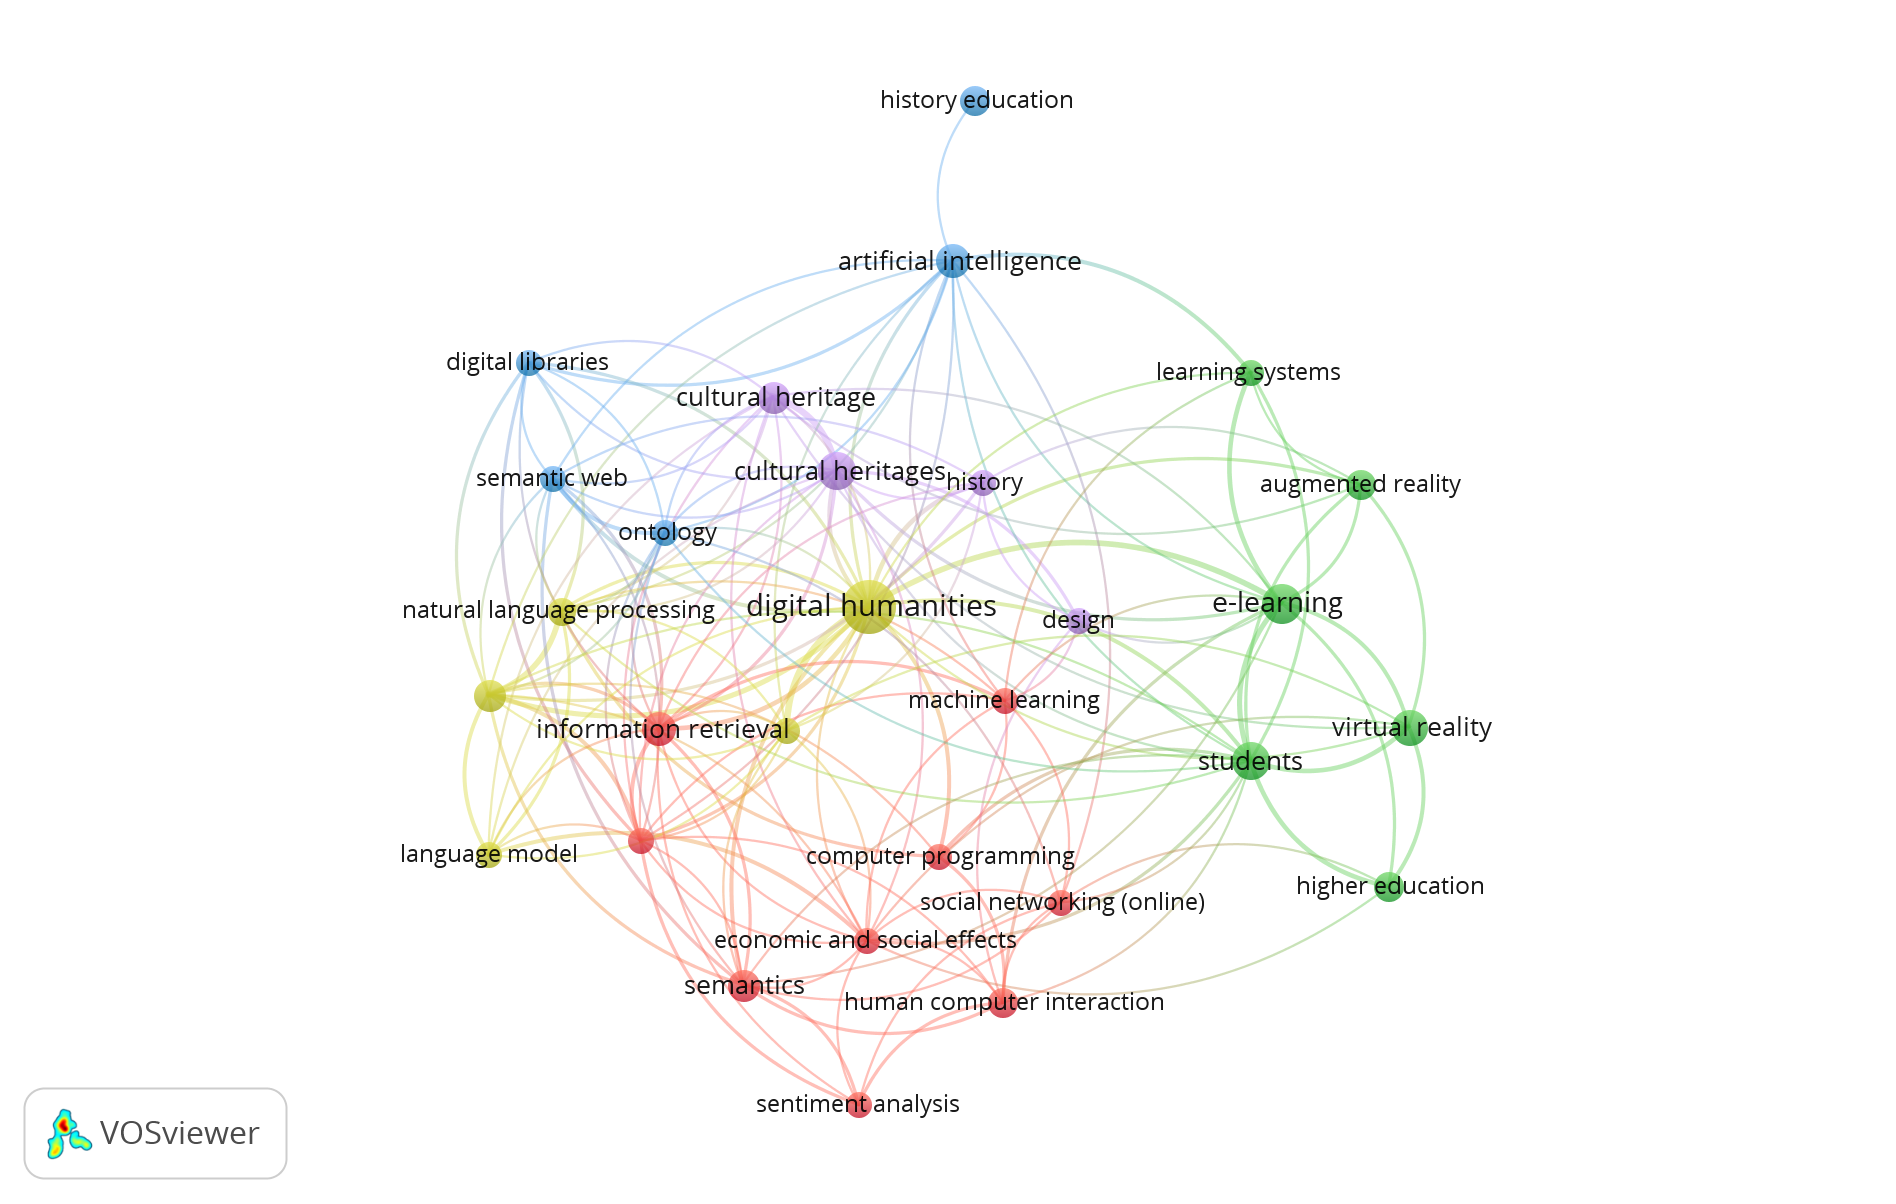
\includegraphics[width=1\linewidth]{data/map_terms.png}
    \caption{Concepts general network}
%    \caption{A holistic view of all clusters.}
    \label{fig:aims_result}
\end{figure}

%Key-words: digital history, teaching, methodology, future professional

The emergence of digital technologies in historical education has created unprecedented opportunities for pedagogical innovation, yet the field remains characterized by significant theoretical and methodological gaps. Through network analysis utilizing VOSviewer software, this study examined 28 key concepts across five distinct clusters to identify critical research lacunae in digital history teaching methodology. The analysis reveals fundamental disconnections between technological capabilities and pedagogical implementation, highlighting the urgent need for comprehensive theoretical frameworks that can bridge these domains.

%The first cluster "digital humanities" (yellow claster) has the greatest strength of communications in 21 lsnks with 58 link strength. It has connection with language analysis, and the most powerful correlation with the concepts of "language processing systems" they are related to the larger concepts of the others. A possible reason for this is that, Digital history it is aprooach of historycal science, and machine language analyse it's a part of this aproach.

%The concepts of "cultural heritages" or "cultural heritage" (purpule claster) and "history" have 26, 20 and 12 connection accordingly. The concept of "cultural heritages" is connected with mostly all the concepts of the blue and yellow clusters and partly with the red claster (there are no connections with the concepts of programming theme). This can be explained by the fact that, heritages are more humanitarian, and about cultural comprehension.

%The concepts of "artifical inteligence"  and "history education" it's the part of blue claster, but placed apart. "Ontology" are connected with all the concepts of the blue cluster, and in the semantic theme. 
%Red claster represent social networking and "human computer ineraction". "Higer education" represents in this cluster with strong convergence "students" and "virtual reality"
%Thus, the concepts of the first cluster ("digital humanites", yellow) have the most connections with the third ("information retreval", red) and fourth ("e-learning", green) clusters.

The emergence of digital technologies in historical education has created unprecedented opportunities for pedagogical innovation, yet the field remains characterized by significant theoretical and methodological gaps. Through network analysis utilizing VOSviewer software, this study examined 28 key concepts across five distinct clusters to identify critical research lacunae in digital history teaching methodology. The analysis reveals fundamental disconnections between technological capabilities and pedagogical implementation, highlighting the urgent need for comprehensive theoretical frameworks that can bridge these domains.


The network analysis reveals significant temporal disparities in research development, with average publication years varying considerably across concept areas. Established approaches such as semantics (2019.08) and information retrieval (2019.78) contrast sharply with emerging technologies like language models (2023.22) and economic and social effects analysis (2023.33). This temporal gap indicates insufficient research attention to integrating rapidly evolving artificial intelligence technologies with established digital history practices.
The emergence of large language models and advanced AI technologies presents both opportunities and challenges for historical education that remain largely unaddressed in current literature. The absence of ethical and methodological frameworks for AI integration represents a critical research gap that could significantly impact the future development of digital history pedagogy.

While cultural heritage concepts demonstrate strong internal clustering and connectivity, their translation into effective teaching methodologies remains underdeveloped. The network analysis shows limited bridges between heritage digitization efforts and practical educational applications, suggesting that preservation-focused initiatives are not adequately informing pedagogical practice.
This disconnect represents a missed opportunity to leverage substantial investments in cultural heritage digitization for educational purposes. Without research frameworks that can effectively translate heritage preservation into teaching resources, significant digital collections may remain underutilized in educational contexts.

The distinct clustering pattern observed in the network analysis reflects broader challenges in cross-disciplinary collaboration between computer science and history education. The minimal inter-cluster connectivity suggests that sustainable partnership models for integrating technical expertise with pedagogical knowledge remain underdeveloped.
This limitation is particularly significant given the complex skill sets required for effective digital history instruction. The development of digital history teaching methodologies necessitates expertise spanning multiple domains, yet current research approaches appear to operate within disciplinary silos rather than fostering genuine interdisciplinary integration.

The network analysis reveals insufficient attention to assessment methodologies for digital history competencies. While technological tools and student engagement receive research attention, validated frameworks for evaluating learning outcomes in digital history contexts remain underdeveloped. This gap impedes both pedagogical improvement and professional preparation, as educators lack reliable methods for assessing student progress and program effectiveness.
The absence of comprehensive assessment frameworks also limits the ability to conduct longitudinal studies on the effectiveness of digital history teaching methods, perpetuating uncertainty about optimal pedagogical approaches and their long-term impacts on student learning and professional development.

Current research demonstrates limited attention to institutional factors affecting digital history program implementation. The weak connections between "higher education" and digital methodologies suggest insufficient consideration of institutional change management, resource allocation, and sustainability factors that influence program success.
This gap is particularly concerning given the substantial investments required for digital history program development and the complex organizational changes necessary for successful implementation. Without research-informed frameworks for institutional adoption, many digital history initiatives may fail to achieve their pedagogical potential or sustain long-term viability.

The network analysis reveals a fundamental research gap in digital history teaching methodology: the absence of comprehensive, theoretically-grounded frameworks that can effectively integrate advanced digital technologies with history-specific pedagogical principles, professional competency development, and institutional sustainability requirements. This overarching deficit manifests across multiple dimensions, including pedagogical integration, professional development, technological adaptation, cross-disciplinary collaboration, assessment methodology, and institutional implementation.
The identified gaps represent significant opportunities for original scholarly contribution through the development of unified theoretical and methodological frameworks for digital history education. Such frameworks must address the complex interplay between technological capability, pedagogical effectiveness, professional preparation, and institutional sustainability to advance the field beyond its current fragmented state.
Future research in this domain should prioritize the development of integrated approaches that can bridge existing knowledge silos while addressing the practical challenges of preparing future historians for an increasingly digital profession. The successful resolution of these research gaps will be essential for realizing the full educational potential of digital technologies in historical scholarship and instruction.


%змінити 2 і 3 розділи місцями:
%введення > методика > експеримент > обговорення
%позбутися предупередження про результати досілдження (пункт 1.3)
\section{FanFic Systematic analysis of sources for training future specialists using Digital History}
It is this source from Digital History that is most important in the conditions of information transmission and constant hybrid wars in the world. Propaganda is often not limited to political issues, but moves into the environment of science and education. In the case of pseudoscientific ideas, the fight is better organized, precisely because of the constant criticism of the sources by the scientists themselves.
In education, this situation is the opposite, since students spend a minority of their time in the classroom (physical or virtual), and on the open Internet they see many versions of the same fact, usually preferring the simplest, which most often turns out to be manipulation or outright lies
The main idea is for students to learn to criticize sources while creating their own
The education system is directly related to society and its changes. Digital history in pedagogy as an approach is designed to speed up all learning and skill formation processes. Digital history as a tool should be accessible and universal enough for the widest range of education seekers.
All requirements for sources for training future specialists (learning materials and tasks) now receive the next level of requirements: "indirect influence". The transition to education 4.0 \cite{MON} requires the formation of such training courses that will be flexible (individualized approach) and available outside the classroom with a teacher.
In this context, the content of the training course should meet the educational needs of the majority of students without the participation of the teacher.

TwT TwT TwT TwT TwT

That is why the main criteria for digital history sources were highlighted

\begin{enumerate}
\item The resource should clearly identify its author(s) or sponsoring institution to establish credibility and context. Evaluators should consider ``Who is the intended audience of the work? What was the purpose of the work?'' \cite{NCPH2016}, since authoritative backing (a recognized archive, university, or scholarly press) lends trust to the project. This information helps students judge expertise and perspective.
\item The accuracy and factual reliability of the content must be verified. Digital history sources should present well-researched information with evidence or citations supporting factual claims. According to established review standards, reviewers should take into consideration ``accuracy of content'' as a core criterion \cite{NCPH2016}. Unverified or poorly supported statements weaken the source's credibility.
\item The resource should situate itself within broader scholarship and describe its methodology. Evaluators should ask whether it fits into a body of scholarly work and how it uses primary or secondary sources, as recommended by NCPH \cite{NCPH2016}. The site should explain its evidence and reasoning, helping students understand the historiographical context. A thorough project will reference its sources and outline how conclusions were reached.
\item The organization and design of the resource should facilitate ease of use. The site needs clear navigation menus, readable layouts, and an intuitive structure. Reviewers check if the resource is easy to navigate and has an effective design that serves its objectives \cite{NCPH2016}. A well-designed interface lets students focus on content rather than technical hurdles.
\item The project should effectively employ digital media and interactive features. Valuable digital history resources often include tools like searchable databases, interactive maps, or timelines that enhance learning. Evaluators should assess whether the site uses new technologies in ways beyond what print media can offer \cite{NCPH2016}. Engaging interactive elements help students visualize data and explore the past actively.
\item The source should provide clear metadata and citation information. A high-quality digital resource will cite its content and provide bibliographic details for any materials presented. Cohen and Rosenzweig advise that a digital history project be both ``easy-to-use and scholarly,'' preserving historical integrity in presentation \cite{CohenRosenzweig2006}. Proper attribution ensures that students can trace information back to its origins.
\item The longevity of the digital resource is crucial for future use. Evaluators should consider whether the project has a preservation plan, such as repository deposit or use of sustainable formats. Cohen and Rosenzweig note that without such measures, even major projects can disappear from the web \cite{CohenRosenzweig2006}. Loss of online content undermines teaching if students cannot access materials in the future.
\item The resource should support pedagogical goals by engaging users in historical inquiry. It should provide contextual introductions or interpretive essays that guide student analysis. Seefeldt and Clark explain that digital history should create a framework for users to ``experience, read, and follow an argument about a major historical problem'' \cite{SeefeldtClark2009}. Effective teaching resources often include guided questions or activities to deepen critical engagement.
\end{enumerate}

Criteria to assess the level of skills will be the final level of knowledge, skills and skills

A comprehensive checklist for developing a quality assessment framework for digital history teaching methodology APPENDIX \ref{frmw_chklst}
 
 \subsubsection{Competency Development Frameworks}

The implementation of technical competency development in digital history education requires sophisticated pedagogical approaches that integrate theoretical understanding with practical application. Competency-based assessment strategies must address both technical proficiency and critical thinking skills, ensuring that practitioners can not only operate digital tools but also evaluate their epistemological implications for historical research.

Assessment frameworks should incorporate portfolio-based evaluation, peer review processes, and authentic assessment strategies that mirror professional digital history practice. This includes the development of rubrics that address both technical execution and scholarly interpretation, ensuring that competency development serves broader historiographical objectives.

\subsubsection{Interdisciplinary Collaboration and Communication} 

Digital history practice increasingly requires competency in interdisciplinary collaboration, including the ability to communicate effectively with computer scientists, librarians, and information professionals. Technical competencies include familiarity with project management methodologies, version control systems for collaborative development, and documentation standards that facilitate interdisciplinary cooperation.

Practitioners must develop competency in technical communication, including the ability to articulate requirements for digital tool development and to evaluate technical solutions against historiographical objectives. Understanding of agile development methodologies and user-centered design principles represents an essential component of collaborative digital history practice.

\subsubsection{Conclusion and Future Directions}

The technical competency framework presented in this analysis represents a comprehensive approach to understanding the skills required for effective digital history practice. As digital technologies continue to evolve, this framework must remain flexible and responsive to emerging tools and methodologies while maintaining focus on fundamental principles of historical scholarship.

Future research should address the development of assessment instruments for measuring competency acquisition, the creation of professional development pathways for practicing historians, and the integration of technical competency development with broader historiographical training. The success of digital history as both a research methodology and pedagogical approach depends upon the systematic development of technical competencies that serve and enhance traditional historical scholarship rather than replacing it.

The framework established herein provides a foundation for curriculum development, professional training, and quality assurance in digital history practice, ensuring that the integration of digital technologies into historical research maintains the rigor and interpretive sophistication that characterizes the discipline at its best.


\subsubsection{Critical Evaluation of Sources}
Hands-On Experience: Providing students with practical experience through projects that involve the use of digital tools and methodologies. 
This includes creating digital archives, developing digital exhibitions, and using digital storytelling to present historical narratives

Case Studies and Simulations: Utilizing case studies and simulations to provide real-world scenarios where students can apply their skills in systematic analysis and critical evaluation of digital sources \cite{Milligan}

\subsubsection{Digital Literacy and Technical Skills}
Navigating Digital Archives: Students are trained to effectively navigate digital archives and databases, using advanced search techniques and understanding metadata to locate relevant historical documents

Using Digital Tools: This includes training in the use of specific digital tools such as Geographic Information Systems (GIS) for mapping historical data, text mining tools for analyzing large text corpora, and data visualization software to represent historical data graphically \cite{Milligan}

\subsubsection{Methodological Approaches}
Source Criticism: Applying traditional historical methodologies to digital sources, such as cross-referencing multiple sources to verify information and constructing a source’s provenance to trace its history and changes over time

Digital Source Management: Teaching students how to manage digital sources effectively, including data storage, organization, and ensuring the long-term preservation of digital materials \cite{Milligan}

Educational Data base

\subsubsection{Theoretical Framework for Competency Development}
The competency progression model presented herein employs a scaffolded learning approach that recognizes the iterative and interconnected nature of skill development in digital history. Drawing upon Bloom's taxonomy and situated learning theory, this framework conceptualizes competency development as a progression from foundational digital literacy through advanced methodological expertise, ultimately culminating in innovative research leadership and pedagogical competency.
The progression model acknowledges that digital history competencies develop neither in isolation nor in strict linear sequences. Rather, competency acquisition follows a spiral curriculum model where learners revisit fundamental concepts at increasingly sophisticated levels of analysis and application. This approach reflects the interdisciplinary nature of digital history, which requires continuous integration of technical skills with historiographical understanding.
APPENDIX \ref{modl_tech_skill}

\subsubsection{Theoretical Foundation for Assessment in Digital History}

The assessment of digital history competencies requires a multifaceted approach that evaluates both technical proficiency and historiographical understanding. This framework employs authentic assessment principles, recognizing that digital history skills are best evaluated through real-world applications that mirror professional practice. The assessment tools presented here integrate formative and summative evaluation strategies, emphasizing process documentation alongside final products to capture the iterative nature of digital scholarship.
Assessment in digital history must address the unique challenges posed by rapidly evolving technologies while maintaining focus on enduring principles of historical inquiry. The framework employs competency-based assessment strategies that allow for multiple pathways to demonstrate mastery, recognizing diverse learning styles and career trajectories within the field
APPENDIX \ref{ass_tool}

\subsubsection{Theoretical Foundation for Benchmark Development}

The establishment of skill benchmarks in digital history requires a sophisticated understanding of competency development that balances technical proficiency with historiographical sophistication. This framework employs criterion-referenced assessment principles, establishing absolute standards of performance rather than relative comparisons. The benchmarks presented here reflect the iterative and interconnected nature of digital history competencies, recognizing that skills develop through progressive mastery rather than discrete achievement levels.
The benchmark framework integrates Miller's Pyramid of Clinical Competence (Knows, Knows How, Shows How, Does) adapted for digital history contexts, ensuring that assessment captures both theoretical understanding and practical application. This approach acknowledges that digital history competency requires not only technical skill execution but also critical evaluation of methodological choices and their historiographical implications.
APPENDIX \ref{compt_msrmnt}

 Analysis of Digital History Pedagogical Approaches

\subsubsection {Overview of Current Approaches}

The document presents a comprehensive framework for digital history education that addresses the challenges of information transmission in an era of "constant hybrid wars" and widespread misinformation. The pedagogical approach is designed to prepare students for Education 4.0 requirements while maintaining rigorous historical scholarship standards.

\subsubsection {Key Pedagogical Frameworks Identified}

\subsubsection {1. Competency-Based Learning Framework}

**Approach:** The document employs a scaffolded learning model based on Bloom's taxonomy and situated learning theory, progressing from foundational digital literacy to advanced methodological expertise.

**Strengths:**
- Recognizes the iterative and interconnected nature of skill development
- Employs a spiral curriculum model where concepts are revisited at increasing levels of sophistication
- Integrates technical skills with historiographical understanding
- Allows for multiple pathways to demonstrate mastery

**Areas for Development:**
- Could benefit from more explicit learning objectives at each competency level
- Needs clearer progression markers between foundational and advanced stages
- Would benefit from peer assessment integration within the competency framework

\subsubsection {2. Source Criticism and Evaluation Methodology}

**Approach:** Eight comprehensive criteria for evaluating digital history sources, emphasizing authorship verification, accuracy, methodology transparency, and pedagogical effectiveness.

**Strengths:**
- Provides concrete, actionable criteria for source evaluation
- Addresses both technical and scholarly dimensions
- Emphasizes the importance of metadata and citation practices
- Considers long-term preservation and accessibility

**Areas for Development:**
- Could include more guidance on evaluating AI-generated or algorithmically-curated content
- Needs stronger emphasis on bias detection in digital platforms
- Would benefit from case studies demonstrating application of these criteria

\subsubsection {3. Authentic Assessment Strategy}

**Approach:** Portfolio-based evaluation, peer review processes, and authentic assessment that mirrors professional digital history practice.

**Strengths:**
- Emphasizes real-world application over theoretical knowledge
- Integrates formative and summative evaluation strategies
- Documents process alongside final products
- Recognizes diverse learning styles and career trajectories

**Areas for Development:**
- Could provide more specific rubrics for different types of digital history projects
- Needs clearer guidelines for peer review processes
- Would benefit from industry partnership integration for authentic assessment

\subsubsection {4. Hands-On Experiential Learning}

**Approach:** Practical projects including digital archive creation, digital exhibitions, and digital storytelling, supplemented by case studies and simulations.

**Strengths:**
- Provides concrete application opportunities
- Develops both technical and creative skills
- Mirrors professional practice in digital humanities
- Encourages active learning and engagement

**Areas for Development:**
- Could benefit from more structured reflection components
- Needs clearer connection between individual projects and broader historical themes
- Would be enhanced by community engagement and public history components

\subsubsection {Critical Analysis of Pedagogical Effectiveness}

\subsubsection {Strengths of the Overall Approach}

1. **Holistic Integration:** The framework successfully integrates technical competencies with traditional historical scholarship, avoiding the trap of treating digital tools as mere add-ons to historical education.

2. **Critical Thinking Emphasis:** Strong focus on source criticism and evaluation skills, which are particularly crucial in the digital age where misinformation proliferates rapidly.

3. **Interdisciplinary Collaboration:** Recognition that digital history requires collaboration across disciplines, preparing students for complex professional environments.

4. **Flexibility and Adaptability:** The framework acknowledges rapid technological change and builds in mechanisms for adaptation while maintaining core historical principles.

\subsubsection {Areas Requiring Enhancement}

1. **Student Agency and Self-Direction:** While the framework mentions individualized approaches, it could better emphasize student choice and self-directed learning pathways.

2. **Cultural and Global Perspectives:** The approach could benefit from more explicit attention to diverse cultural contexts and non-Western approaches to digital history.

3. **Ethical Framework Development:** While ethics are mentioned, a more comprehensive ethical reasoning framework could be integrated throughout the curriculum.

4. **Public Engagement:** Greater emphasis on public history and community engagement could enhance the relevance and impact of student work.

\subsubsection Recommendations for Pedagogical Improvement

\subsubsection 1. Enhanced Metacognitive Components
- Integrate regular reflection activities that help students understand their own learning processes
- Develop self-assessment tools that complement instructor and peer evaluation
- Create learning journals that document both successes and challenges in digital history work

\subsubsection 2. Community-Centered Learning
- Establish partnerships with local historical societies, museums, and community organizations
- Design projects that address real community needs and historical questions
- Integrate public presentation and community feedback into assessment strategies

\subsubsection 3. Cross-Cultural and Global Perspectives
- Include case studies from diverse global contexts
- Address issues of digital divide and technological access
- Examine how different cultures approach digitization and historical preservation

\subsubsection 4. Advanced Ethical Reasoning
- Develop scenario-based ethical decision-making exercises
- Address contemporary issues like deepfakes, AI-generated content, and digital manipulation
- Include discussions of power dynamics in digital archiving and representation

\subsubsection 5. Innovation and Research Leadership
- Create opportunities for students to identify and address gaps in existing digital history tools
- Encourage experimental approaches to digital storytelling and presentation
- Foster entrepreneurial thinking about digital history applications

\subsubsection Conclusion

The pedagogical framework presented demonstrates sophisticated understanding of digital history education needs. Its strength lies in the integration of technical competencies with traditional historical scholarship while maintaining flexibility for emerging technologies. However, the approach would benefit from greater emphasis on student self-direction, cultural diversity, community engagement, and advanced ethical reasoning.

The framework provides a solid foundation for digital history education but requires ongoing refinement to address the rapidly evolving landscape of digital tools, changing student needs, and emerging ethical challenges in the digital humanities field.

\subsection{Ethical Considerations}

 Ethical Considerations in Digital History: Contemporary Research and Framework

\subsubsection Current Ethical Landscape in Digital History

Based on recent research, digital history faces unprecedented ethical challenges that extend far beyond the traditional concerns of privacy and copyright mentioned in the original document. The integration of AI and machine learning into digital humanities has introduced new layers of complexity requiring sophisticated ethical frameworks.

\subsubsection Core Ethical Domains

\subsubsection 1. Digital Preservation Ethics

**Contemporary Challenges:**
- Digital material is often deleted or replaced before a preservationist can act, creating unique temporal pressures
- Copyright laws create challenging tasks for preservationists working with digital materials
- Recent DMCA rulings have denied exemptions for digital preservation, limiting institutional preservation efforts

**Key Considerations:**
- Balancing access rights with copyright protection
- Establishing protocols for orphaned digital works
- Addressing the ephemeral nature of digital content
- Managing preservation responsibilities across institutional boundaries

\subsubsection 2. AI and Algorithmic Bias

**Emerging Concerns:**
- Algorithmic bias is potentially a major social and cultural crisis for humanity
- AI systems have produced racially biased outputs based on unbalanced training datasets
- Digital humanities projects risk perpetuating historical biases through visualization and data representation

**Critical Issues:**
- Training data reflects historical inequities and underrepresentation
- Algorithmic decision-making in archival selection and curation
- Bias amplification in search algorithms and recommendation systems
- Cultural asymmetries in AI development and application

\subsubsection 3. Cultural Representation and Power Dynamics

**Contemporary Research Findings:**
- Limited and distorted representation in AI systems creates philosophical and technical challenges
- AI integration into humanities offers new tools but requires careful consideration of cultural heritage preservation
- Digital archives often reflect the perspectives and priorities of dominant cultural groups

**Ethical Imperatives:**
- Ensuring diverse voices in digital collection development
- Addressing historical silences and absences in digitized materials
- Recognizing community ownership of cultural materials
- Implementing inclusive metadata and cataloging practices

\subsubsection 4. Privacy and Consent in Digital Archives

**Evolving Challenges:**
- New ethical concerns are introduced as AI becomes prevalent, raising questions about where to draw the line
- Posthumous privacy rights for digitized personal materials
- Consent for materials created before digital preservation was anticipated
- Balancing research access with individual privacy protection

**Consideration Areas:**
- Retroactive consent for historical materials
- Privacy implications of searchable full-text databases
- Data mining and pattern analysis of personal communications
- Cross-cultural concepts of privacy and public access

\subsubsection Institutional and Legal Framework Analysis

\subsubsection Copyright and Legal Compliance

Current legal frameworks struggle to address digital preservation needs:
- Statutory requirements including public records legislation and Freedom of Information Act expectations apply to digital records
- Retention requirements often conflict with preservation goals
- Fair use doctrine application to digital preservation remains unclear
- International copyright variations complicate global digital projects

\subsubsection Professional Ethics Standards

The field lacks comprehensive ethical guidelines that address:
- Responsibility hierarchies between institutions, researchers, and communities
- Standards for AI-assisted research and analysis
- Guidelines for handling culturally sensitive materials
- Protocols for addressing discovered biases in existing digital collections

\subsubsection Recommendations for Ethical Framework Development

\subsubsection 1. Comprehensive Ethics Training

**For Educators:**
- Integrate bias recognition and mitigation training
- Develop case study curricula addressing real ethical dilemmas
- Establish partnerships with affected communities
- Create assessment tools for ethical decision-making competency

**For Students:**
- Mandatory ethics components in all digital history courses
- Practical exercises in identifying and addressing bias
- Community engagement requirements
- Reflection portfolios documenting ethical reasoning development

\subsubsection 2. Institutional Policy Development

**Core Policy Areas:**
- AI use guidelines for research and teaching
- Community consultation protocols for sensitive materials
- Bias audit procedures for digital collections
- Transparent correction and amendment processes

**Implementation Strategies:**
- Ethics review boards for digital humanities projects
- Regular policy updates reflecting technological changes
- Community advisory boards with meaningful decision-making power
- Public reporting on ethical practices and challenges

\subsubsection 3. Technical Solutions with Ethical Oversight

**Algorithm Development:**
- Bias detection and mitigation tools for digital collections
- Transparent AI decision-making processes
- Diverse training datasets for AI applications
- Community input in algorithm design and testing

**Access and Interface Design:**
- Multiple perspective presentation of controversial materials
- Contextual warnings for potentially biased or harmful content
- User empowerment through customizable filters and searches
- Accessibility compliance ensuring equitable access

\subsubsection 4. Community-Centered Approaches

**Engagement Strategies:**
- Co-creation of digital projects with represented communities
- Community ownership models for cultural materials
- Benefit-sharing agreements for commercialized research
- Regular community feedback and project adjustment mechanisms

**Representation Considerations:**
- Diverse hiring in digital history projects
- Community training programs for digital skills
- Indigenous data sovereignty principles
- Culturally appropriate metadata and description practices

\subsubsection Future Directions and Research Needs

\subsubsection Emerging Ethical Challenges

**Technological Developments:**
- Deepfake technology implications for historical evidence
- Blockchain and NFT applications to cultural materials
- Virtual and augmented reality ethical considerations
- Quantum computing implications for privacy and security

**Social and Political Considerations:**
- Digital colonialism and cultural appropriation
- Platform monopolization of cultural content
- Government surveillance through cultural databases
- Climate change impact on digital preservation ethics

\subsubsection Research Priorities

1. **Empirical Studies:** Long-term impact assessments of current ethical practices
2. **Cross-Cultural Research:** Comparative studies of ethical frameworks globally
3. **Technical Development:** Bias detection and mitigation tool effectiveness
4. **Community Impact:** Evaluation of community-centered digital history projects
5. **Policy Analysis:** Effectiveness of current legal and institutional frameworks

\subsubsection Conclusion

The ethical landscape of digital history has evolved significantly beyond the basic privacy and copyright concerns identified in traditional frameworks. While numerous ethical frameworks and principles have been created, the majority lack operationalization and standardization. 

Contemporary challenges require integrated approaches addressing AI bias, cultural representation, community rights, and evolving legal frameworks. Educational programs must move beyond awareness-building to develop practical competencies in ethical reasoning and community engagement.

The success of ethical digital history practice depends on ongoing collaboration between technologists, historians, communities, and policymakers to develop responsive, inclusive, and accountable approaches to digital cultural heritage work.

\subsection{Interdisciplinary Collaboration}

 Collaboration Frameworks for Digital History Education

\subsubsection Overview

Based on contemporary research and best practices, this document presents comprehensive collaboration frameworks designed to address the interdisciplinary nature of digital history while fostering meaningful partnerships between academics, communities, and technical professionals.

\subsubsection Core Collaboration Models

\subsubsection 1. Transdisciplinary Integration Framework

**Theoretical Foundation:**
Transdisciplinarity contrasts with interdisciplinary and multidisciplinarity in the sense that the former is transformative, while interdisciplinarity is concerned with linking and integrating, and multidisciplinarity juxtaposes different approaches.

**Implementation Structure:**
- **Shared Conceptual Framework Development**: Creating unified vocabularies and methodologies across disciplines
- **Transformative Research Goals**: Projects that fundamentally alter understanding rather than simply combining approaches
- **Cross-Disciplinary Mentorship**: Rotating leadership and expertise sharing
- **Integrated Assessment**: Evaluation criteria that value transformation over traditional disciplinary outputs

**Key Components:**
- Joint curriculum development between computer science, history, and library science
- Shared laboratory spaces for collaborative experimentation
- Cross-training programs for faculty and students
- Integrated research projects with shared intellectual ownership

\subsubsection 2. Community-Academic Partnership Framework

**Philosophical Approach:**
We invite work at the intersections of critical DH, that engages with anti-colonial and post-colonial frameworks, that supports feminist and anti-racist praxis, and that crosses political and disciplinary borders.

**Partnership Structure:**
- **Community Advisory Boards**: Local stakeholders with decision-making authority
- **Co-Creation Processes**: Shared project design and implementation
- **Capacity Building**: Training programs for community members in digital skills
- **Benefit Sharing**: Explicit agreements about project outcomes and intellectual property

**Implementation Elements:**
- Community needs assessment protocols
- Participatory research methodologies
- Cultural competency training for academic partners
- Sustainable funding models that support long-term relationships
- Public presentation and feedback mechanisms

\subsubsection 3. Technical-Humanistic Collaboration Framework

**Core Principle:**
Computer scientists need to be open to humanities' hermeneutic traditions and engage in the interpretative and contextualization processes of humanities research more deeply.

**Collaboration Structure:**
- **Embedded Partnerships**: Computer scientists working within humanities research contexts
- **Interpretative Engagement**: Technical team participation in historical interpretation
- **Process-Oriented Development**: Process-oriented thinking that takes the opportunities as well as limits of computational and digitization processes into account
- **Digital Hermeneutics**: Digital hermeneutics provides a potential framework for bridging technical and interpretative work

**Operational Elements:**
- Joint training workshops for technical and humanities teams
- Shared documentation practices that include both technical specifications and interpretative frameworks
- Iterative development cycles with regular humanities feedback
- Cross-disciplinary evaluation criteria for technical solutions

\subsubsection 4. Institutional Collaboration Framework

**Multi-Institutional Approach:**
It involved multiple forms of collaboration: cross-sectoral (between the British Library and university partners in London and Oxford); international (between UK institutions and Aarhus University in Denmark); and interdisciplinary (between the Oxford Internet Institute and the Institute of Historical Research, University of London).

**Framework Components:**
- **Cross-Sector Partnerships**: Libraries, universities, cultural institutions, and community organizations
- **International Collaboration**: Global perspectives and resource sharing
- **Infrastructure Sharing**: Technical resources, expertise, and data management
- **Coordinated Programming**: Aligned educational and research initiatives

**Implementation Strategy:**
- Formal partnership agreements with clear roles and responsibilities
- Shared governance structures with rotating leadership
- Joint funding applications and resource allocation
- Regular partnership evaluation and adjustment mechanisms

\subsubsection Pedagogical Collaboration Strategies

\subsubsection 1. Collaborative Learning Environments

**Physical and Virtual Spaces:**
- Libraries need to be open for outside involvement: They could provide spaces for collaboration, engage in interdisciplinary projects when digitizing their archival collections, and help fund experiments
- Maker spaces equipped with both traditional research tools and digital technologies
- Virtual collaboration platforms for distributed teams
- Community-accessible workshop spaces

**Learning Activities:**
- Team-based research projects with mixed disciplinary groups
- Peer teaching and learning exchanges
- Community-based learning experiences
- International collaboration projects

\subsubsection 2. Mentorship and Training Models

**Multi-Directional Mentorship:**
- Senior academics mentoring junior researchers across disciplines
- Community experts mentoring academic researchers
- Students mentoring peers in specialized skills
- International mentorship exchanges

**Professional Development:**
- Cross-disciplinary skill-building workshops
- Community engagement training
- Technical literacy development for humanities scholars
- Cultural competency training for technical professionals

\subsubsection 3. Assessment and Evaluation Frameworks

**Collaborative Assessment Strategies:**
- Portfolio-based evaluation including multiple perspectives
- Community feedback integration
- Peer review processes across disciplines
- Self-reflection and metacognitive assessment
- Impact measurement including community benefits

**Quality Assurance:**
- Multi-stakeholder evaluation committees
- Regular project review and adjustment processes
- Transparent feedback mechanisms
- Continuous improvement protocols

\subsubsection Addressing Collaboration Challenges

\subsubsection 1. Power Dynamics and Hierarchy Issues

**Problem Recognition:**
Not discussing human-human collaborations is also a way of implying a "them" and "us" structure of academe where different categories of contributors occupy different and hierarchized spaces.

**Solutions:**
- Explicit discussion of power dynamics in collaboration agreements
- Rotating leadership roles across partners
- Equal compensation and recognition for all contributors
- Decision-making processes that ensure all voices are heard

\subsubsection 2. Communication and Language Barriers

**Multi-Language Support:**
- Translation services for international collaborations
- Technical vocabulary training for humanities scholars
- Humanities methodology training for technical professionals
- Community language accessibility measures

**Communication Protocols:**
- Regular check-in meetings with structured agendas
- Shared documentation systems accessible to all partners
- Multiple communication channels (formal and informal)
- Conflict resolution procedures

\subsubsection 3. Sustainability and Long-Term Viability

**Financial Sustainability:**
- Diversified funding strategies including grants, institutional support, and community contributions
- Clear budget allocation and financial responsibility agreements
- Revenue-sharing models where appropriate
- Long-term funding relationship development

**Intellectual Sustainability:**
- Knowledge transfer protocols ensuring continuity
- Documentation systems that preserve institutional memory
- Succession planning for key personnel
- Skills development programs for ongoing capacity building

\subsubsection Implementation Guidelines

\subsubsection Phase 1: Foundation Building (Months 1-6)
- Partner identification and initial relationship building
- Shared vision and goal development
- Resource assessment and allocation planning
- Initial training and capacity building activities

\subsubsection Phase 2: Collaborative Development (Months 7-18)
- Joint project design and implementation
- Regular feedback and adjustment cycles
- Skill sharing and cross-training programs
- Community engagement and feedback integration

\subsubsection Phase 3: Sustainability and Expansion (Months 19+)
- Long-term relationship formalization
- Impact assessment and evaluation
- Model replication and scaling strategies
- Network expansion and new partnership development

\subsubsection Evaluation Metrics

\subsubsection Quantitative Measures
- Number of successful collaborative projects completed
- Participant satisfaction ratings across all stakeholder groups
- Skill development assessments for all participants
- Community impact measurements
- Academic output and recognition metrics

\subsubsection Qualitative Measures
- Depth of cross-disciplinary understanding demonstrated
- Quality of community relationships and trust building
- Innovation and creativity in collaborative approaches
- Sustainability of partnerships over time
- Transformation of institutional practices and cultures

\subsubsection Future Directions

\subsubsection Emerging Collaboration Models
- AI-assisted collaboration tools and platforms
- Virtual and augmented reality collaborative environments
- Blockchain-based collaboration and attribution systems
- Global network collaboration frameworks

\subsubsection Research and Development Needs
- Empirical studies of collaboration effectiveness
- Cultural adaptation of collaboration frameworks
- Technology development for enhanced collaboration
- Policy development supporting collaborative work

\subsubsection Conclusion

Effective collaboration in digital history education requires intentional framework development that addresses power dynamics, cultural differences, technical barriers, and sustainability challenges. Success depends on commitment to equitable partnership, ongoing communication, and adaptive approaches that evolve with changing needs and contexts.

The frameworks presented here provide structured approaches while maintaining flexibility for local adaptation and innovation. Their implementation requires institutional commitment, adequate resources, and genuine commitment to transformative collaborative practice.

\subsection{Practical Application and Projects}
Hands-On Experience: Providing students with practical experience through projects that involve the use of digital tools and methodologies. This includes creating digital archives, developing digital exhibitions, and using digital storytelling to present historical narratives.

Case Studies and Simulations: Utilizing case studies and simulations to provide real-world scenarios where students can apply their skills in systematic analysis and critical evaluation of digital sources \cite{Milligan} .

\subsection{Technical skill requarimments}

 Technical Competency Framework for Digital History Methodologies: A Comprehensive Analysis of Required Skill Sets for Advanced Historical Research

\subsubsection Introduction

The integration of digital technologies into historical research and pedagogy necessitates a comprehensive framework for understanding the technical competencies required for effective utilization of digital history tools. This analysis establishes a taxonomic structure of technical skills that addresses the multifaceted nature of digital historical inquiry, encompassing both foundational digital literacy and advanced methodological applications. The framework presented herein responds to the increasing complexity of digital history as both a pedagogical approach and a research methodology, reflecting the transition to Education 4.0 paradigms that demand flexible, individualized, and technology-enhanced learning environments.

\subsubsection Theoretical Foundation and Methodological Context

Digital history, as conceptualized within contemporary historiographical discourse, represents a convergence of traditional historical methodologies with computational approaches to data analysis, visualization, and preservation. The technical competency framework developed in this study builds upon established principles of source criticism while extending these methodologies to address the unique challenges presented by digital materials and tools. This approach aligns with the scholarly consensus that digital history should maintain historiographical rigor while leveraging technological capabilities to enhance analytical depth and accessibility.

\subsubsection Core Technical Competency Domains

\subsubsection 1. Advanced Information Retrieval and Database Management

The foundational layer of digital history competency encompasses sophisticated information retrieval skills that extend beyond basic search capabilities. Practitioners must demonstrate proficiency in advanced query construction, utilizing Boolean operators, field-specific searches, and controlled vocabulary systems. Metadata literacy represents a critical component of this domain, requiring understanding of Dublin Core, MODS (Metadata Object Description Schema), and specialized historical metadata standards. Database navigation skills must encompass both relational and non-relational database structures, with particular emphasis on understanding the architectural principles underlying major historical repositories and digital collections.

The complexity of contemporary digital archives demands expertise in cross-platform searching techniques, federated search methodologies, and API utilization for programmatic access to collections. Practitioners must develop competency in evaluating database architecture and understanding how organizational schemes affect discoverability and research outcomes. This includes familiarity with controlled vocabularies, taxonomies, and ontologies specific to historical domains.

\subsubsection 2. Computational Analysis and Visualization Technologies

\subsubsection {Geographic Information Systems (GIS) for Historical Analysis}

Spatial analysis capabilities represent a fundamental requirement for contemporary digital historians. GIS competency encompasses not merely operational knowledge of software platforms, but theoretical understanding of spatial analysis principles, coordinate systems, and projection methodologies. Historical GIS applications require specialized skills in georeferencing historical cartographic materials, temporal data modeling, and the creation of spatiotemporal databases that can accommodate the uncertainty and ambiguity inherent in historical spatial data.

Advanced practitioners must demonstrate competency in spatial statistics, network analysis, and the integration of qualitative historical evidence with quantitative spatial models. This includes understanding the epistemological implications of spatial analysis in historical contexts and the ability to critically evaluate the limitations and assumptions underlying GIS-based historical arguments.

\subsubsection Computational Text Analysis and Digital Humanities Methods

Text mining and computational linguistics represent increasingly central components of digital history practice. Required competencies include familiarity with natural language processing techniques, named entity recognition, topic modeling, and sentiment analysis as applied to historical corpora. Practitioners must understand the principles of corpus preparation, including text cleaning, normalization, and the handling of historical linguistic variations and orthographic inconsistencies.

Advanced text analysis requires proficiency in statistical software environments (R, Python) and specialized digital humanities tools (Voyant, AntConc, MALLET). Practitioners must develop critical awareness of the interpretive challenges posed by computational text analysis, including issues of representativeness, bias in digitized collections, and the relationship between quantitative patterns and qualitative historical interpretation.

\subsubsection Data Visualization and Information Design

Effective communication of historical research through digital media requires sophisticated visualization competencies. This encompasses both technical proficiency in visualization software (D3.js, Tableau, Gephi) and theoretical understanding of information design principles. Historical data visualization presents unique challenges related to temporal representation, uncertainty visualization, and the integration of qualitative and quantitative evidence.

Practitioners must demonstrate competency in interactive visualization design, understanding user experience principles, and the creation of scholarly visualizations that maintain analytical rigor while enhancing accessibility. This includes knowledge of accessibility standards (WCAG guidelines) and universal design principles for inclusive digital scholarship.

\subsubsection 3. Digital Asset Management and Preservation

\subsubsection Long-term Digital Preservation Strategies

Digital preservation competency encompasses understanding of preservation metadata standards (PREMIS), digital repository architecture, and format migration strategies. Practitioners must demonstrate familiarity with preservation planning methodologies, risk assessment for digital materials, and the implementation of preservation workflows that ensure long-term accessibility of digital historical resources.

Technical requirements include knowledge of sustainable file formats, checksum verification procedures, and version control systems. Advanced practitioners must understand the relationship between preservation strategies and scholarly access, including the development of preservation policies that balance long-term sustainability with immediate research needs.

\subsubsection Data Management and Interoperability

Effective digital history practice requires sophisticated data management competencies, including database design principles, data modeling for historical information, and interoperability standards. Practitioners must demonstrate proficiency in metadata crosswalking, format conversion, and the implementation of linked data principles for historical resources.

Technical competencies include familiarity with XML schemas, RDF/SPARQL for linked data applications, and API development for data sharing. Understanding of FAIR (Findable, Accessible, Interoperable, Reusable) data principles represents an essential component of contemporary digital history practice.

\subsubsection 4. Web Technologies and Digital Publishing

\subsubsection Platform Development and Content Management

Digital history increasingly requires competency in web development technologies, including HTML5, CSS3, and JavaScript for creating interactive historical presentations. Content management system (CMS) proficiency encompasses both end-user competency and understanding of system architecture, customization capabilities, and security considerations.

Advanced practitioners must demonstrate understanding of responsive design principles, cross-browser compatibility, and web accessibility standards. This includes knowledge of version control systems (Git), collaborative development workflows, and deployment strategies for digital history projects.

\subsubsection Digital Exhibition and Narrative Technologies

The creation of compelling digital historical narratives requires proficiency in multimedia integration, interactive storytelling platforms, and user experience design. Technical competencies include familiarity with content delivery networks, multimedia optimization, and the integration of various media types within coherent narrative structures.

Practitioners must understand the relationship between technological capabilities and historiographical objectives, ensuring that digital presentation strategies enhance rather than compromise scholarly rigor and interpretive complexity.

\subsubsection Critical Evaluation and Quality Assurance Competencies

\subsubsection Digital Source Criticism and Authentication

Digital history practice demands sophisticated source criticism competencies that address the unique challenges posed by digital materials. This includes understanding of digital forensics principles, provenance tracking for digital objects, and the evaluation of authenticity in digital contexts. Practitioners must develop competency in cross-referencing digital sources, evaluating the reliability of digitization processes, and understanding the implications of digital mediation for historical evidence.

Technical skills include familiarity with metadata analysis, digital watermarking, and version control systems that enable tracking of changes to digital historical materials. Understanding of blockchain technologies for provenance verification represents an emerging competency area for digital historians.

\subsubsection Ethical Frameworks and Compliance

Digital history practice operates within complex ethical and legal frameworks that require specialized competencies. Practitioners must demonstrate understanding of copyright law as applied to digital historical materials, privacy considerations for digitized personal documents, and the ethical implications of computational analysis of historical texts and images.

Technical competencies include familiarity with digital rights management systems, anonymization techniques for sensitive historical data, and compliance frameworks for international data sharing. Understanding of indigenous data sovereignty principles and community-based ethical frameworks represents an increasingly important competency area.


Key-Frame Design for Digital History Educational Course
Course Title: "Critical Digital History: Methods, Ethics, and Practice"
Course Overview
This course prepares students to engage critically with digital historical methods while developing technical competencies and ethical reasoning skills. The curriculum integrates traditional historiographical training with contemporary digital tools, emphasizing collaborative practice and community engagement.
Learning Objectives
By course completion, students will demonstrate ability to evaluate digital historical sources using established criteria, apply digital tools appropriately to historical research questions, collaborate effectively across disciplinary boundaries, articulate ethical considerations in digital history practice, and create original digital history projects that serve both scholarly and public audiences.
Course Structure (15-week semester)
Module 1: Foundations and Critical Framework (Weeks 1-3)
Week 1 introduces the information landscape and digital literacy fundamentals. Students examine how misinformation proliferates in digital environments and learn basic principles of source criticism adapted for digital contexts. Practical activities include analyzing social media posts claiming historical "facts" and identifying reliable digital archives.
Week 2 focuses on digital history as both methodology and tool. Students explore the difference between digitized historical materials and born-digital sources, understanding how digitization processes affect historical interpretation. Hands-on work includes comparing physical documents with their digital reproductions and examining metadata structures.
Week 3 establishes ethical frameworks for digital history practice. Students engage with contemporary debates about algorithmic bias, cultural representation, and community rights in digital archives. Activities include case study analysis of controversial digitization projects and development of personal ethical guidelines.
Module 2: Technical Competencies and Source Evaluation (Weeks 4-7)
Week 4 develops advanced digital archive navigation skills. Students learn sophisticated search strategies, understand metadata schemas, and practice using finding aids in major digital repositories. Technical work includes creating comprehensive search strategies for specific research questions.
Week 5 focuses on the eight-criteria framework for digital source evaluation. Students apply criteria systematically to various digital history resources, learning to assess authorship, accuracy, methodology, design, digital features, metadata, longevity, and pedagogical value. Practical application involves evaluating and ranking digital history websites.
Week 6 introduces basic digital tools including Geographic Information Systems for historical mapping, text analysis software for document corpora, and data visualization tools. Students complete guided tutorials and small-scale projects demonstrating tool competency.
Week 7 emphasizes methodological transparency and documentation. Students learn version control systems, collaborative documentation practices, and research data management. Practical work includes creating project documentation that could be reproduced by other researchers.
Module 3: Collaborative Practice and Community Engagement (Weeks 8-10)
Week 8 establishes frameworks for interdisciplinary collaboration. Students engage in simulated collaboration exercises with computer science and library science students, learning to communicate across disciplinary boundaries and manage collaborative workflows.
Week 9 focuses on community-academic partnerships. Local community representatives guest lecture about their historical preservation needs. Students begin identifying potential community partners for final projects and learn protocols for respectful community engagement.
Week 10 develops skills in cultural competency and inclusive practice. Students examine case studies of successful and problematic community collaborations, learning to recognize power dynamics and develop equitable partnership approaches.
Module 4: Advanced Applications and Critical Analysis (Weeks 11-13)
Week 11 explores artificial intelligence applications in digital history. Students examine AI-assisted research tools, learn to identify algorithmic bias, and practice transparent documentation of AI tool usage in research.
Week 12 focuses on digital storytelling and public presentation. Students learn principles of effective digital narrative construction, accessibility design, and audience engagement strategies for public history contexts.
Week 13 addresses digital preservation and long-term sustainability. Students understand preservation challenges, learn about sustainable file formats, and explore institutional repository systems for ensuring long-term access to digital history projects.
Module 5: Synthesis and Application (Weeks 14-15)
Weeks 14-15 are dedicated to final project presentations and peer review. Students present completed digital history projects, engage in structured peer feedback sessions, and reflect on their learning progression throughout the course.
Assessment Strategy
Continuous Assessment (40%)
Weekly reflection journals document students' evolving understanding of digital history concepts and ethical considerations. Source evaluation exercises require students to apply the eight-criteria framework to various digital resources. Collaboration participation is assessed through peer evaluation and self-reflection on group work contributions.
Mid-term Portfolio (25%)
Students compile a portfolio demonstrating technical competency development, including documented experiments with digital tools, successful completion of search strategies, and evidence of collaborative skill development. Portfolio includes reflective analysis connecting technical skills to historiographical understanding.
Final Community-Engaged Project (35%)
Students work individually or in small teams to complete digital history projects addressing real community needs. Projects must demonstrate technical competency, ethical reasoning, collaborative practice, and effective communication to public audiences. Assessment criteria include community feedback, technical execution, historical accuracy, and reflective analysis of the collaborative process.
Pedagogical Innovations
Spiral Learning Implementation
Concepts are introduced simply and revisited with increasing complexity. For example, source criticism begins with basic website evaluation and progresses to sophisticated analysis of algorithmic bias in search results and database construction.
Authentic Assessment Integration
All assignments mirror real professional practice in digital history. Students work with actual community partners, use professional-grade tools, and create projects suitable for public presentation or institutional use.
Multiple Perspective Integration
Each major topic is examined from at least three perspectives: technical/methodological, ethical/social, and historical/interpretative. This ensures students develop comprehensive understanding rather than purely instrumental skill.
Community Partnership Implementation
Local Historical Society Collaboration
Partnership with regional historical societies provides authentic project opportunities. Students work on actual digitization needs, website development, or public programming support under professional supervision.
Cultural Institution Engagement
Museums, libraries, and cultural centers serve as both learning laboratories and project sites. Students gain exposure to professional digital history practice while contributing meaningful work to institutional goals.
International Collaboration
Sister relationships with international institutions provide global perspectives on digital history practice and expose students to different cultural approaches to digitization and preservation.
Technology and Infrastructure Requirements
Physical Learning Spaces
Flexible classroom space accommodating both traditional seminar discussion and hands-on technical work. Access to presentation technology supporting multiple simultaneous group work sessions.
Digital Platform Access
Institutional subscriptions to major digital archive collections, professional-grade software tools for text analysis and mapping, and collaborative platform access for group project management.
Community Access Support
Resources for students to meet with community partners, transportation support for site visits, and technology lending program ensuring all students can participate regardless of personal device access.
Continuous Improvement Mechanisms
Regular Feedback Integration
Mid-semester course adjustments based on student feedback and learning assessment. Community partner input shapes project requirements and collaboration protocols.
Professional Development Alignment
Annual review of curriculum alignment with emerging professional standards and technological developments. Regular consultation with digital history practitioners ensures course relevance.
Research Integration
Course serves as laboratory for ongoing research into digital history pedagogy effectiveness. Student work contributes to understanding of best practices in digital history education.
Expected Outcomes
Students completing this course will be prepared for advanced digital history research, equipped with practical skills for digital humanities careers, and capable of ethical, collaborative practice in community-engaged historical work. The course design ensures graduates can navigate rapidly changing technological landscapes while maintaining commitment to rigorous historical scholarship and community accountability.
This framework balances technical skill development with critical thinking, ethical reasoning, and collaborative practice, preparing students for the complex demands of contemporary digital history practice while fostering lifelong learning capabilities essential for success in rapidly evolving digital environments.RetryClaude can make mistakes. Please double-check responses. Sonnet 4Chat controls Sonnet 4Smart, efficient model for everyday use Learn moreArtifactsAnalysis o

%ПЕРЕПИСАТИ ↓ ↓ ↓ ↓
% in Wiki +
Current scholarship discusses the evolution and challenges of the digital humanities, noting its shift to "digital methods," but emphasizing the need for a broader understanding beyond just tools, highlighting historians' concerns about the impact of digitization on access, copyright, ethics, and recognition and appreciation digital scholarship, and the need to teach and assess digital skills in history education \cite{Brennan}.
    
%ПЕРЕПИСАТИ ↓ ↓ ↓ ↓
% in Wiki +
Attempts are also being made to introduce digital history as an emerging field utilizing digital technology and computational methods, inviting global collaboration and offering innovative ways to explore, understand, and represent the past, with Hannu Salmi's work providing a comprehensive introduction encompassing its origins, basic concepts, interdisciplinary nature, public engagement, challenges, and focus on the contemporary age's digital transformation. \cite{salmi}

%ПЕРЕПИСАТИ ↓ ↓ ↓ ↓
% in Wiki +
Also takes place discusses the ongoing digital transformation in historical scholarship, showcasing a collection of research in "Digital Histories" that utilizes digital and computational methods across various historical periods and geographic regions, highlighting the shift towards generating new historical knowledge while addressing the challenges and limitations posed by digital tools and emphasizing the importance of digital source criticism. \cite{fridlund}

%ПЕРЕПИСАТИ ↓ ↓ ↓ ↓
% in Wiki +
The topic of Digital History is also presented in methodological literature, such as a comprehensive teacher's guide that contains design principles and practical strategies for integrating digital history into college and high school courses, emphasizing the potential of digital tools and methods to enrich historical pedagogy and promote the accessibility of historical narratives\cite{guiliano}.

%Проекти з ЦІ ↓ ↓ ↓ ↓



    %advice for creating a title: Be brief and avoid wasting words
Digital History: Teaching Methodology 
    %pose the topic as a brief question

Digital History: what already exists?

    % if investigators have resources to collect data

    %what the topic adds to the pool of research knowledge available on the topic, replicates past studies, lifts up the voices of underrepresented groups or individuals, helps address social justice, or transforms the ideas and beliefs of the researcher

    %How does this project contribute to the literature?



